\chapter{EXPERIMENTAL RESULTS}
Precision and recall are two metrics used to evaluate classification and retrieval systems' performance. Precision is the percentage of relevant occurrences among all retrieved examples. Recall, also known as sensitivity, is the percentage of recovered instances among all appropriate models. In a perfect classifier, precision and recall are both one. Object detection models like YOLO use the assessment measure mAP (mean Average Precision). To calculate mAP, we needed IOU, Precision, Recall, Precision Recall Curve, and AP.\\
The YOLOv4 model training took more time compared to YOLOv5 and YOLOv56. The model achieved the overall mAP of 98.68\%. Below table shows the overall result on YOLOv4 training. 
\begin{table}[H]
\caption{YOLOv4 Results}
\centering
\begin{tabular}{llllll} 
\cline{1-3}
\multicolumn{1}{|l|}{\textcolor[rgb]{0.141,0.125,0.129}{Class}}                               & \multicolumn{1}{l|}{\textcolor[rgb]{0.141,0.125,0.129}{Average Precision}} & \multicolumn{1}{l|}{\textcolor[rgb]{0.141,0.125,0.129}{mAP@0.50}}                                                                      &  &  &   \\ 
\cline{1-3}
\multicolumn{1}{|l|}{\textcolor[rgb]{0.141,0.125,0.129}{Visible change without cavitation}}   & \multicolumn{1}{l|}{\textcolor[rgb]{0.141,0.125,0.129}{96.61\%}}           & \multicolumn{1}{l|}{\textcolor[rgb]{0.141,0.125,0.129}{~} \textcolor[rgb]{0.141,0.125,0.129}{~} \textcolor[rgb]{0.141,0.125,0.129}{~}} &  &  &   \\ 
\cline{1-2}
\multicolumn{1}{|l|}{\textcolor[rgb]{0.141,0.125,0.129}{Visible change with microcavitation}} & \multicolumn{1}{l|}{\textcolor[rgb]{0.141,0.125,0.129}{99.85\%}}           & \multicolumn{1}{l|}{~ ~\textcolor[rgb]{0.141,0.125,0.129}{98.68 \%}}                                                                   &  &  &   \\ 
\cline{1-2}
\multicolumn{1}{|l|}{\textcolor[rgb]{0.141,0.125,0.129}{Visible change with cavitation}}      & \multicolumn{1}{l|}{\textcolor[rgb]{0.141,0.125,0.129}{100.00\%}}          & \multicolumn{1}{l|}{}                                                                                                                  &  &  &   \\ 
\cline{1-3}
 
\end{tabular}
\end{table}
For conf thresh = 0.25, precision = 0.97, recall = 0.96, F1-score = 0.97. Again, For conf thresh = 0.25, TP = 285, FP = 8, FN = 12, average IoU = 79.60\%. IoU threshold = 50\%, used Area-Under-Curve for each unique Recall. Mean average precision (mAP@0.50) = 0.988213, or 98.82\%. Total Detection Time: 1 Seconds\\
The YOLOv5s model was trained with 100 epoch and outperformed the YOLOv4 models. The model achieved the precision of 97.8\% on overall class. mAP@.5 was 98.9\% and mAP@.5:.95 was 76.7\%. The classwise result for YOLOv5 is given below:
\begin{table}[H]
\caption{YOLOv5 Results}
\centering
\begin{tabular}{|l|l|l|l|l|l} 
\cline{1-5}
\textcolor[rgb]{0.141,0.125,0.129}{Class}                               & \textcolor[rgb]{0.141,0.125,0.129}{Precision} & \textcolor[rgb]{0.141,0.125,0.129}{Recall} & \textcolor[rgb]{0.141,0.125,0.129}{mAP@.5} & \textcolor[rgb]{0.141,0.125,0.129}{mAP@.5:.95} &   \\ 
\cline{1-5}
\textcolor[rgb]{0.141,0.125,0.129}{All}                                 & \textcolor[rgb]{0.141,0.125,0.129}{97.8\%}    & \textcolor[rgb]{0.141,0.125,0.129}{98\%}   & \textcolor[rgb]{0.141,0.125,0.129}{98.9\%} & \textcolor[rgb]{0.141,0.125,0.129}{76.7\%}     &   \\ 
\cline{1-5}
\textcolor[rgb]{0.141,0.125,0.129}{Visible change without cavitation}   & \textcolor[rgb]{0.141,0.125,0.129}{99.3\%}    & \textcolor[rgb]{0.141,0.125,0.129}{95.8\%} & \textcolor[rgb]{0.141,0.125,0.129}{98\%}   & \textcolor[rgb]{0.141,0.125,0.129}{72.4\%}     &   \\ 
\cline{1-5}
\textcolor[rgb]{0.141,0.125,0.129}{Visible change with microcavitation} & \textcolor[rgb]{0.141,0.125,0.129}{95.3\%}    & \textcolor[rgb]{0.141,0.125,0.129}{98.2\%} & \textcolor[rgb]{0.141,0.125,0.129}{99.1\%} & \textcolor[rgb]{0.141,0.125,0.129}{76.1\%}     &   \\ 
\cline{1-5}
\textcolor[rgb]{0.141,0.125,0.129}{Visible change with cavitation}      & \textcolor[rgb]{0.141,0.125,0.129}{98.9\%}    & \textcolor[rgb]{0.141,0.125,0.129}{100\%}  & \textcolor[rgb]{0.141,0.125,0.129}{99.6\%} & \textcolor[rgb]{0.141,0.125,0.129}{81.6\%}     &   \\ 
\cline{1-5}
\end{tabular}
\end{table}
The model YOLOv6 on the other hand, was trained with 100 epoch and outperformed slightly compared to YOLOv5. The model achieved an accuracy of 99.24\%. The classwise result for YOLOv6 is given below:
\begin{table}[H]
\caption{YOLOv6 Results}
\centering
\begin{tabular}{|l|l|l|l|} 
\hline
\textcolor[rgb]{0.141,0.125,0.129}{Class}                               & \begin{tabular}[c]{@{}l@{}}\textcolor[rgb]{0.141,0.125,0.129}{Precision} \\\textcolor[rgb]{0.141,0.125,0.129}{@.5:.95}\end{tabular} & \textcolor[rgb]{0.141,0.125,0.129}{Recall@.5:.95} & \textcolor[rgb]{0.141,0.125,0.129}{mAP@.5}   \\ 
\hline
\textcolor[rgb]{0.141,0.125,0.129}{ALL}                                 & \textcolor[rgb]{0.141,0.125,0.129}{88.4\%}                                                                                          & \textcolor[rgb]{0.141,0.125,0.129}{91.3\%}        &                                              \\ 
\cline{1-3}
\textcolor[rgb]{0.141,0.125,0.129}{Visible change without cavitation}   & \textcolor[rgb]{0.141,0.125,0.129}{100\%}                                                                                           & \textcolor[rgb]{0.141,0.125,0.129}{100\%}         & \textcolor[rgb]{0.141,0.125,0.129}{99.24\%}  \\ 
\cline{1-3}
\textcolor[rgb]{0.141,0.125,0.129}{Visible change with microcavitation} & \textcolor[rgb]{0.141,0.125,0.129}{83.7\%}                                                                                          & \textcolor[rgb]{0.141,0.125,0.129}{84.8\%}        &                                              \\ 
\cline{1-3}
\textcolor[rgb]{0.141,0.125,0.129}{Visible change with cavitation}      & \textcolor[rgb]{0.141,0.125,0.129}{88.8\%}                                                                                          & \textcolor[rgb]{0.141,0.125,0.129}{91.8\%}        &                                              \\
\hline
\end{tabular}
\end{table}
YOLOv6's result is generated as a json file. So, Only graphical results of YOLOv5 is shown below: 
\begin{figure}[H]
    \centering
    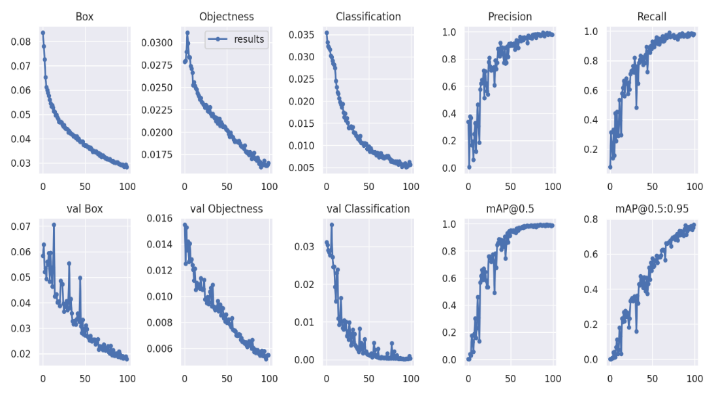
\includegraphics[scale=1.8]{55_chapter_5/y1.png}
    \caption{Result of training in YOLOv5}
    \label{YOLOv5s}
\end{figure}
\begin{figure}[H]
    \centering
    \includegraphics[scale=1{55_chapter_5/y2.png}
    \caption{Recall curve for YOLOv5}
    \label{YOLOv5s}
\end{figure}
\begin{figure}[H]
    \centering
    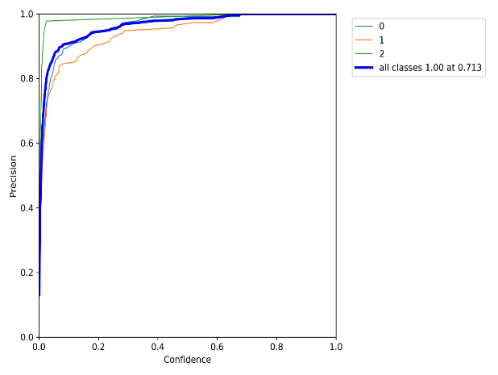
\includegraphics[scale=1]{55_chapter_5/y3.png}
    \caption{Precision curve for YOLOv5}
    \label{YOLOv5s}
\end{figure}
\begin{figure}[H]
    \centering
    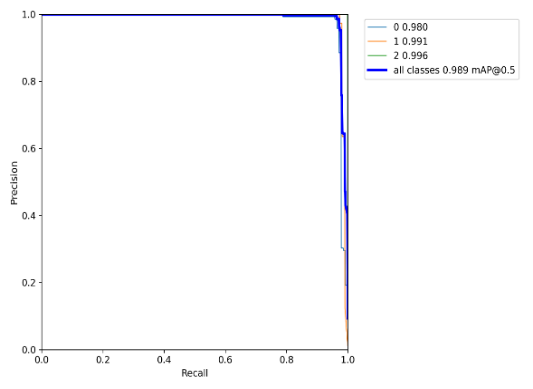
\includegraphics[scale=1]{55_chapter_5/y4.png}
    \caption{Precision-Recall curve for YOLOv5}
    \label{YOLOv5s}
\end{figure}
\begin{figure}[H]
    \centering
    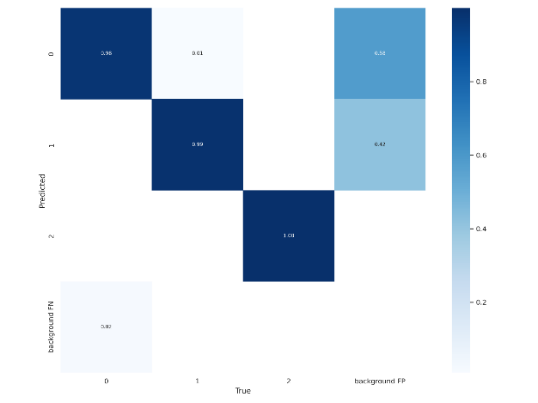
\includegraphics[scale=1]{55_chapter_5/y5.png}
    \caption{Confusion matrix for YOLOv5}
    \label{YOLOv5s}
\end{figure}
\begin{figure}[H]
    \centering
    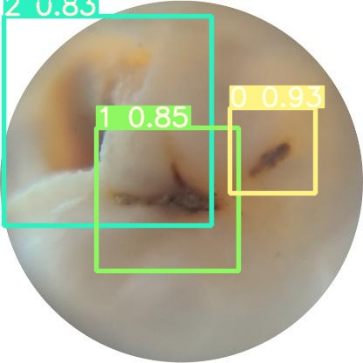
\includegraphics[scale=1]{55_chapter_5/y6.png}
    \caption{Sample Output of YOLOv5 model }
    \label{YOLOv5s}
\end{figure}
All of the above model train in same environment (Google Colab) with almost same condition. So, we can compare their mAP and time in a graph for better visualization.\
\begin{figure}[H]
    \centering
    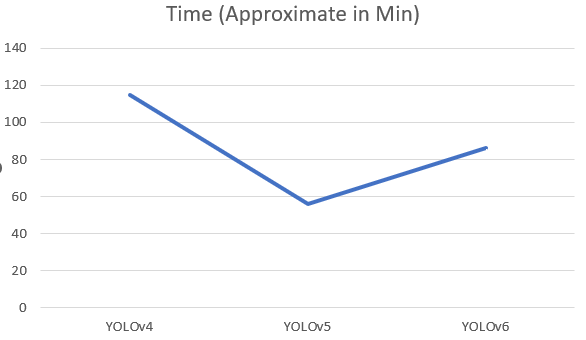
\includegraphics[scale=1]{55_chapter_5/g1.png}
    \caption{Model VS Time}
    \label{Graph}
\end{figure}
\begin{figure}[H]
    \centering
    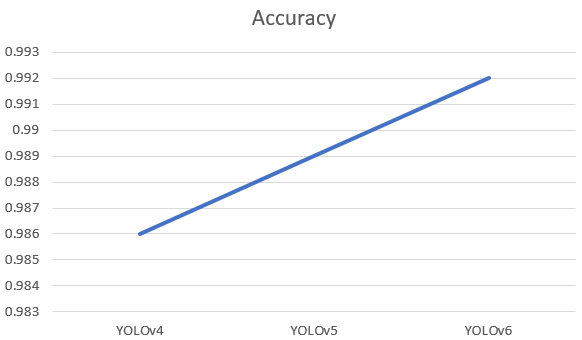
\includegraphics[scale=1]{55_chapter_5/g2.png}
    \caption{Model VS mAP@0.5}
    \label{Graph}
\end{figure}